% Copyright (C) 2013 Kevin W. Hamlen
%
% This program is free software; you can redistribute it and/or
% modify it under the terms of the GNU General Public License
% as published by the Free Software Foundation; either version 2
% of the License, or (at your option) any later version.
%
% This program is distributed in the hope that it will be useful,
% but WITHOUT ANY WARRANTY; without even the implied warranty of
% MERCHANTABILITY or FITNESS FOR A PARTICULAR PURPOSE.  See the
% GNU General Public License for more details.
%
% You should have received a copy of the GNU General Public License
% along with this program; if not, write to the Free Software
% Foundation, Inc., 51 Franklin Street, Fifth Floor, Boston,
% MA  02110-1301, USA.
%
% The latest version of this program can be obtained from
% http://songs.sourceforge.net.
%
\documentclass[12pt,oneside,letterpaper]{article}
\usepackage[bookmarks]{hyperref}
\usepackage{songs}
\usepackage{graphicx}

\songcolumns{0}
\renewcommand\songtarget[2]{}
\renewcommand\songlink[2]{#2}

\setlength{\oddsidemargin}{0in}
\setlength{\evensidemargin}{0in}
\setlength{\textwidth}{6.5in}
\setlength{\topmargin}{0in}
\setlength{\topskip}{0in}
\setlength{\headheight}{0in}
\setlength{\headsep}{0in}
\setlength{\textheight}{8.5in}

\newcommand{\vimversion}{72}
\newcommand{\miktexversion}{2.7}

\newcommand{\mytt}{\tt\chardef\{="7B\chardef\}="7D\relax}
\newcommand{\ppath}[1]{{\mytt#1}}
\newcommand{\fslash}{\char"5C\relax}
\newcommand{\songpath}{Songbook\fslash}
\newcommand{\texbase}{C:\fslash Program Files\fslash MiKTeX \miktexversion}
\newcommand{\localbase}{C:\fslash localtexmf}
\newcommand{\vimbase}{C:\fslash Program Files\fslash Vim}
\newcommand{\texpath}{\texbase\fslash tex\fslash latex\fslash}
\newcommand{\tfmpath}{\localbase\fslash fonts\fslash tfm\fslash ms\fslash }
\newcommand{\vfpath}{\localbase\fslash fonts\fslash vf\fslash ms\fslash}
\newcommand{\vimpath}{\vimbase\fslash vimfiles\fslash}

\newcommand{\ltx}[1]{{\mytt#1}}
\newcommand{\lesc}{\char"5C\relax}
\definecolor{ltxmac}{rgb}{0.5,0.25,0.25}
\definecolor{ltxopt}{rgb}{1,0,1}
\definecolor{ltxcmd}{rgb}{0.625,0.125,0.9375}
\definecolor{ltxfnt}{rgb}{0.18,0.543,0.34}
\definecolor{ltxcmt}{rgb}{0,0,1}
\definecolor{ltxdel}{rgb}{0.414,0.3516,0.8}
\definecolor{sbdsng}{rgb}{0,0,0.5}
\definecolor{sbdcmd}{rgb}{0.414,0.352,0.8}
\definecolor{sbdvrs}{rgb}{1,0.312,0}
\definecolor{sbdcrd}{rgb}{0.18,0.543,0.34}
\definecolor{sbdmbr}{rgb}{0.5,0.25,0.25}
\definecolor{sbdif}{rgb}{1,0,0}
\definecolor{sbdscr}{rgb}{0.625,0.125,0.9375}
\definecolor{sbdlig}{rgb}{0.414,0.352,0.8}
\newcommand{\schord}[1]{\ltx{\textcolor{sbdcrd}{\lesc[#1]}}}
\newcommand{\slyric}[2]{\ltx{\textcolor{sbdcrd}{\lesc[#1]}#2}}
\newcommand{\spcrd}[1]{\ltx{\textcolor{sbdcrd}{#1}}}
\newcommand{\smbar}{\ltx{\textcolor{sbdmbr}{|}}}
\newcommand{\scmd}[1]{\ltx{\textcolor{sbdcmd}{#1}}}
\newcommand{\sbeg}[1]{\ltx{\textcolor{sbdsng}{#1}}}
\newcommand{\sverse}[1]{\ltx{\textcolor{sbdvrs}{#1}}}
\newcommand{\scond}[1]{\ltx{\textcolor{sbdif}{#1}}}
\newcommand{\serror}[1]{\colorbox{red}{\kern-2pt\ltx{#1}\kern-2pt}}
\newcommand{\swarn}[1]{\colorbox{yellow}{\kern-2pt\ltx{#1}\kern-2pt}}
\newcommand{\slig}[1]{\colorbox{sbdlig}{\kern-2pt\ltx{#1}\kern-2pt}}
\newcommand{\smac}[1]{\ltx{\textcolor{ltxmac}{\lesc#1}}}
\newcommand{\sdel}[1]{\ltx{\textcolor{ltxdel}{#1}}}
\newcommand{\sopt}[1]{\ltx{\textcolor{ltxopt}{#1}}}

\newenvironment{bsexample}{%
  \noindent\hfil\vbox\bgroup%
    \hsize3in\versesep=5pt\vskip1pt\setcounter{songnum}{1}%
}{%
  \egroup\par%
}

\renewcommand\thefootnote{\fnsymbol{footnote}}
\newcommand{\example}[1]{{\hangindent=1in\hangafter=1\parindent=0.5in{#1}\par}}
\newbox\exbox
\newdimen\exboxadj
\newcommand{\vctr}[1]{%
  \exboxadj=0.5\ht\exbox%
  \advance\exboxadj by#1\relax%
  \lower\exboxadj\box\exbox%
}
\newcommand{\bscr}{%
  \vspace{5pt}%
  \begingroup%
    \def\prodpad{\hss}%
    \setbox\exbox=\vbox\bgroup\begingroup%
      \parindent=0pt\mytt\small\color{sbdscr}%
}
\newcommand{\withscr}{%
    \endgroup\egroup%
    \produces{\vctr{-4pt}}%
    \setbox\exbox=\vbox\bgroup%
      \parindent=0.13in%
      \hsize=2.5in%
}
\newcommand{\escr}{%
    \egroup%
    \vctr{-4pt}%
  \endgroup%
  \par%
}
\newcommand{\tabexample}[2]{{%
  \produces{\scmd{\lesc gtab\{#1\}\{#2\}}}%
  \hsize=1.4in%
  \setbox\exbox=\vbox{\gtab{#1}{#2}}%
  \vctr{-12pt}%
}}

\makeatletter
  \newcommand\likeverse{\SB@insongtrue\SB@inversetrue}
  \newcommand\unverse{\SB@insongfalse\SB@inversefalse}
  \SB@loadactives
\makeatother

\newcommand\bigmch[4]{{\baselineskip=24pt\mch{#1}{#2}{#3}{#4}}}

\newlength\prodlen
\setlength{\prodlen}{2.8in}
\newcommand{\prodpad}{\hfil}
\newcommand{\produces}[1]{%
	\noindent\hspace*{0.3in}%
	\vbox{\hbox to\prodlen{\ltx{#1}\prodpad}}%
	\ {\it produces}\quad%
}
\newcommand\sampmbar{{\baselineskip=20pt\measurebar}}
\newcommand\sampmeter[2]{{\baselineskip=20pt\mbar{#1}{#2}}}
\newcommand\sampmch[4]{\baselineskip=20pt\mch{#1}{#2}{#3}{#4}}


\begin{document}
\vspace*{1cm}\hfil{\Huge Creating Song Books}\par\vspace{1cm}

This README file provides an introductory explanation of how to use the Songs
\LaTeX\ package on Windows.
It is intended as a user-friendly tutorial for those not already familiar
with the \LaTeX\ document-publishing system.
If you are already familiar with \LaTeX\ or you are a Unix user, you will
probably find the official package documentation more helpful than this
document.
The official package documentation can be found online at
\href{http://songs.sourceforge.net}{songs.sourceforge.net}.

\section{Installing}\label{sec:installing}

To install the song book software on Windows, run the \ppath{setup}
self-installer available for download at
\href{http://songs.sourceforge.net}{songs.sourceforge.net}.

\section{Compiling the Song Book}\label{sec:compiling}

After you've completed the installation, locate the \ppath{Songbook} folder
on your desktop (or elsewhere if you changed the default directory during
installation), and open the \ppath{Sample} subfolder inside.
Double-click the \ppath{songs.sbd} icon.
The Vim file editor window will open.

\vspace{-8pt}\noindent{\hsize=3in\vtop{\parfillskip=0pt\kern0pt %
Near the top of the window you will see a row of icons.
One of them (usually the fourth one from the left) will show a green arrow
pointing rightward to a reddish document with the tiny letters ``PDF'' in it.
If you hover the mouse pointer over it, the words ``Save file and generate a
song book pdf'' will appear over the icon.
Click (with}}%
\hfil\vtop{\kern0pt\hbox to3.2in{\hfil\resizebox{3.2in}{!}{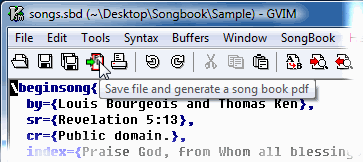
\includegraphics{tbar.png}}}}\par\vspace{2pt}

\noindent
the left mouse button) on that icon.
(If you can't find the proper icon, you can alternatively use the menus.
Open the ``SongBook'' menu and select ``Generate''.)

Once you've either clicked on the correct icon or selected the correct menu
item, a black DOS window will open and lots of text will flow by.
Hopefully it will conclude with the words ``Completed successfully!'' and
prompt you to hit any key to continue.
(If it doesn't, then that means you have edited one of the songbook files
incorrectly and caused an error.
See Section \ref{sec:errors} for instructions on how to diagnose and correct
errors.)
Press any key to close the black DOS window and then close the Vim file editor
window (by clicking on the X-button in the top-right corner of the window).

In the \ppath{Sample} folder you'll now see new files named
\ppath{chordbook.pdf}, \ppath{lyricbook.pdf}, \ppath{slidebook.pdf}, and
\ppath{transparencies.pdf}.
Double-click on any and Adobe Acrobat Reader will open, displaying each newly
created song book.

\section{Common Tasks}\label{sec:common}

\subsection{Creating Handouts}

To create handouts containing only some songs in some particular order, you
must edit the \ppath{chordbook.tex}, \ppath{lyricbook.tex},
\ppath{slidebook.tex}, or \ppath{transparencies.tex} file in the
\ppath{Sample} folder, depending on whether you want a handout for musicians,
a handout for singers, a set of digital projector slides, or a set of
overhead transparencies.
Here's how:

\vspace{-15pt}\noindent\vtop{\hsize=3.45in\hbox{}%
Start by double-clicking on the icon for which\-ever of the above files
you wish to modify.
The Vim file editor program will open and you'll see a lot of \LaTeX\ 
programming.
Find the blue-colored line near the top of the file that starts with the text
``\ltx{\textcolor{ltxcmt}{\%~\lesc includeonlysongs}}''.
The ``\ltx{\textcolor{ltxcmt}{\%}}'' in front of that line tells the song
book generator to ignore that line, so right now it doesn't do anything.
Move the cursor down and remove the ``\ltx{\textcolor{ltxcmt}{\%}}'' and the
space after it.
The line will probably change color to brown to indicate that it is now
active.%
\parfillskip=0pt\par}%
\hfil%
\vtop{\hbox{}\vspace{4pt}\hbox to3in{\hfil\resizebox{3in}{!}{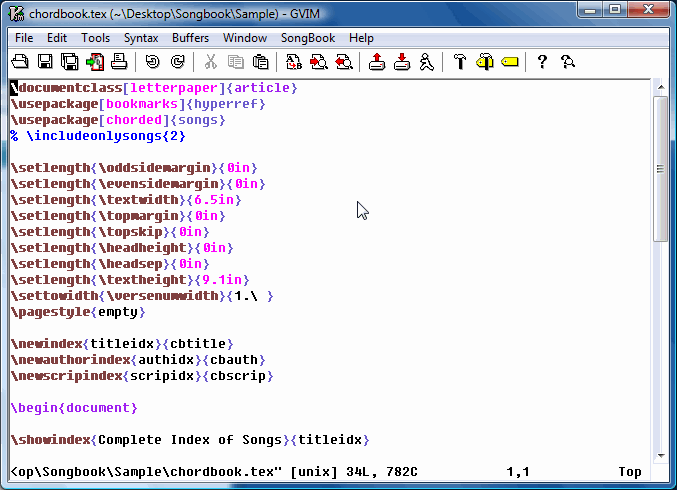
\includegraphics{texshot.png}}}}%
\kern-20pt\par
\vspace{3pt}

\noindent
Immediately after the ``\ltx{\textcolor{ltxmac}{\lesc includeonlysongs}}''
part, you'll see a pair of braces
``\ltx{\textcolor{ltxdel}{\{}} ... \ltx{\textcolor{ltxdel}{\}}}'' enclosing
a comma-separated list of song numbers.
Replace that list with your own list of song numbers in the order you want
them to appear in the handout.
Song numbers should match whatever numbering scheme your song book uses
(e.g., ``\ltx{85,32,128}'' if it uses standard arabic numbering).
Separate the numbers with commas and no spaces.
For example:

\example{\ltx{\textcolor{ltxmac}{\lesc includeonlysongs}\textcolor{ltxdel}{\{}85,32,128\textcolor{ltxdel}{\}}}}

Next, recompile the songbook (see Section \ref{sec:compiling}), and when you
open the pdf file for the tex file that you modified, you'll find a handout
including only the songs you listed.
To go back to a full song book, reinsert the ``\ltx{\textcolor{ltxcmt}{\%}}''
in front of the ``\ltx{\textcolor{ltxmac}{\lesc includeonlysongs}}'' line.


\subsection{Adding New Songs}

\vspace{-15pt}\noindent\vtop{\hsize=3.45in\hbox{}%
To add a new song, go to the \ppath{Sample} folder and double-click on the
icon for \ppath{songs.sbd}.
The Vim file editor will open and you'll see how the sample songs were
entered.
If you want to just jump in and experiment, you can scroll to the bottom of
that file and start typing in a new song the same way you see the other songs
in the file entered.

Vim will automatically color the things that you type in various ways to
indicate whether it thinks they are correct or not.
For example, when you first start typing the word ``\sbeg{\lesc beginsong}'',%
\parfillskip=0pt\par}%
\hfil%
\vtop{\hbox{}\vspace{8pt}\hbox to3in{\hfil\resizebox{3in}{!}{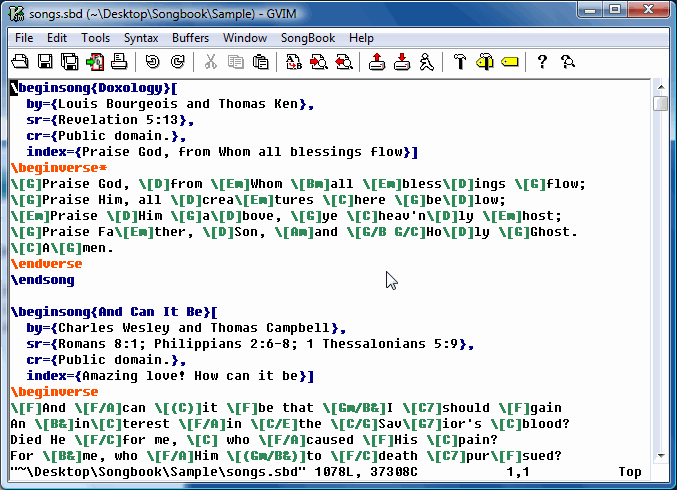
\includegraphics{sbdshot.png}}}}%
\kern-20pt\par
\vspace{3pt}

\noindent it will be in black because Vim
doesn't recognize any command named ``\ltx{\lesc beginso}''.
When you finally hit the last \ltx{g} in ``\sbeg{\lesc beginsong}'', the
entire word will change color to dark blue.

From the sample songs already in the \ppath{songs.sbd} file, you can see how
to write typical songs.
For a more systematic discussion of the various available syntaxes, see
Section \ref{sec:syntax}.

When you're done entering your new song, click on the icon for compiling the
songbook or use the SongBook menu to recompile the song book
(see Section \ref{sec:compiling}).
If no errors are reported, then open \ppath{songbook.pdf} to view your work.
Otherwise see Section \ref{sec:errors} on errors.


\section{Song Entry Syntax}\label{sec:syntax}

For most people it is easier to learn the proper song entry syntax by
example than to read about it in this document.
You can view examples for about twenty public domain songs by 
double-clicking on the icon for \ppath{songs.sbd} in the \ppath{Sample}
folder.
However, if you are trying to do something unusual or would like more
explanation, read on.

\subsection{Structure of a Song}\label{sec:beginsong}

Each song in a songbook begins with a line like:

\example{\ltx{\sbeg{\lesc beginsong\{Title\}[by=\{}Authors\sbeg{\},sr=\{}Scripture refs\sbeg{\},cr=\{}Copyright\sbeg{\}]}}}

\noindent This will produce a song that looks like:

\begin{bsexample}%
\beginsong{Title}[by={Authors},sr={Scripture refs},cr={Copyright}]
\endsong%
\end{bsexample}

\noindent The song number (``1'' in this example) is inferred
automatically---songs are numbered in the order they appear.

The \sbeg{by=\{}\ldots\sbeg{\}},
\sbeg{sr=\{}\ldots\sbeg{\}}, and
\sbeg{cr=\{}\ldots\sbeg{\}} parts may be provided in any order,
and any may be omitted.
You may also type them on separate lines of the input file if you like;
doing so won't affect the appearance of the resulting book.
The ``Title'' part may either be a single song title or multiple song
titles separated by double-backslashes (\sbeg{\lesc\lesc}).
For example,

\example{\sbeg{\lesc beginsong\{Main Title~\lesc\lesc~Second Title\}[}}
\example{\ltx{\ \ \sbeg{cr=\{}\lesc copyright$\sim$\the\year\sbeg{\},}}}
\example{\ltx{\ \ \sbeg{sr=\{}John 3:16\sbeg{\}]}}}

\noindent will produce

\begin{bsexample}%
\beginsong{Main Title \\ Second Title}[cr={\copyright~\the\year},sr={John 3:16}]
\endsong
\end{bsexample}

A separate index entry will be created in each of the book's indexes for
each of the song's titles.
The scripture index will also be affected by anything you put in the
``Scripture refs'' field, and the author index will be affected by
anything you put in the ``Authors'' field.
If you enter an illegal scripture reference for a song (e.g., a
misspelled book of the Bible, a chapter or verse that doesn't
exist, etc.) then an error message will alert you to the problem
when you try to compile the book.

A song ends with the line:

\example{\sbeg{\lesc endsong}}

Between the \sbeg{\lesc beginsong} and \sbeg{\lesc endsong} lines,
a number of constructs are possible in any order desired.
They are...

\subsubsection{Verses}

Start a new verse by issuing the line:

\example{\sverse{\lesc beginverse}}

\noindent Proceed to enter each line of text in the verse (see Section
\ref{sec:contents}).
Then end the verse by issuing the line:

\example{\sverse{\lesc endverse}}

Any number of verses may be in a song.
If you have verse numbering turned on, you can prevent an individual verse
from being numbered by using \sverse{\lesc beginverse*} instead of
\sverse{\lesc beginverse}.
(Use \sverse{\lesc endverse} to end such a verse.)

\subsubsection{Choruses}

Start a chorus by issuing the line:

\example{\sverse{\lesc beginchorus}}

\noindent Enter each line of the chorus exactly as for a verse.
End the chorus by issuing the line:

\example{\sverse{\lesc endchorus}}

There may be any number of choruses in a song. In the generated song book,
a chorus differs from a verse only in that it will be indented and
accompanied by a vertical line in the left margin.
Choruses are also not numbered.

\subsubsection{Musicians' Notes}\label{sec:musicnote}

You can include textual notes that only appear in the musicians' version
by entering:

\example{\scmd{\lesc musicnote\{text of note\}}}

\noindent This command will have no effect upon lyric-only versions of the
book, but will cause the musicians' version to contain text in a shaded box:

\noindent\hspace*{0.5in}\vbox{\advance\hsize-0.5in\musicnote{text of note}\unskip}\par

Musicians' notes should normally only be placed within verses or choruses
or before the first verse/chorus of a song.
It is okay to place them elsewhere between the \sbeg{\lesc beginsong} and
\sbeg{\lesc endsong} lines, but if you do so, they can become separated
from the verse or chorus they refer to by a page or column break.
Never place them between songs.

\label{sec:capo}There is a special kind of musicnote that provides a capo
suggestion for guitarists.
If you put

\example{\scmd{\lesc capo\{1\}}}

\noindent
in a song, it will insert the following textual note in the musicians'
version, suggesting that guitarists put a capo on fret 1:

\noindent\hspace*{0.5in}\vbox{\advance\hsize-0.5in\capo{1}\unskip}\par

\noindent You can replace ``1'' with any number up to 11, but it is
unusual to put a capo on any fret above the 5th one.
The \scmd{\lesc capo} musicnote differs from a regular musicnote,
though, because in a pianists' version of the book, the
\scmd{\lesc capo} musicnote will cause the chords in the song to be
transposed.
See Section \ref{sec:transpose} for how to make a pianists' version
that uses this feature.

\subsubsection{General Notes}

Textual notes to be shown in both the lyric-only and the chorded
versions of the songbook are written as:

\example{\scmd{\lesc textnote\{text of note\}}}

\noindent
They are exactly like musicians' notes (see Section
\ref{sec:musicnote}) except they also appear in the lyric-only
version.

\subsubsection{Extra Index Entries}

You can add additional index entries for the song in two different ways.
To add an index entry corresponding to notable lines from the song's
lyrics, add the following to the list of options in the \sbeg{\lesc beginsong}
line (see Section \ref{sec:beginsong}):

\example{\sbeg{index=\{}\ltx{some short lyrics go here}\sbeg{\}}}

\noindent To add an index entry corresponding to an alternate title
for the song, add:

\example{\sbeg{ititle=\{}\ltx{the alternate title goes here}\sbeg{\}}}

These lines will add an extra entry to every title index related to the
book section in which the song is located.

\subsubsection{Licensing Information}

For your song book to be legal, each song that is not part of the public
domain needs to be used under the auspices of a license purchased by your
organization.
Information about the license under which the song is being used is
generally printed after the copyright information on the copyright line.
You may specify licensing information for the current song by adding the
following to the list of options in the \sbeg{\lesc beginsong} line:

\example{\sbeg{li=\{}\ltx{text to be added after the copyright info}\sbeg{\}}}

Usually the same licensing information is used for many songs, so you will want
to define a macro that abbreviates the licensing info.
For example, if you own a CCLI license, then in the preamble of the
\ppath{songbook.tex} file you could put

\example{\ltx{%
  \textcolor{ltxmac}{\lesc newcommand}\textcolor{ltxdel}{\{}%
  \textcolor{ltxmac}{\lesc CCLI}%
  \textcolor{ltxdel}{\}\{}%
  (CCLI \textcolor{ltxdel}{\lesc\#}123456)%
  \textcolor{ltxdel}{\}\}}%
}}

\noindent
and then in each \sbeg{\lesc beginsong} line for a song covered by CCLI,
you could just put

\example{\sbeg{li=}\ltx{\lesc CCLI}}

\noindent to cause the CCLI license number for your organization to be printed.


For example, the code

\example{\ltx{\sbeg{\lesc beginsong\{Title\}[by=\{}Joe Smith\sbeg{\},sr=\{}Job 3:1-5\sbeg{\},}}}
\example{\ltx{\ \ \ \ \ \ \ \ \ \ \ \ \ \ \ \ \ \ \sbeg{cr=\{}\lesc copyright$\sim$\the\year\ someone\sbeg{\},}}}
\example{\ltx{\ \ \ \ \ \ \ \ \ \ \ \ \ \ \ \ \ \ \sbeg{li=}\lesc CCLI\sbeg{]}}}
\example{\sbeg{\lesc endsong}}

\noindent produces a song like

\begin{bsexample}%
\beginsong{Title}[by={Joe Smith},sr={Job 3:1-5},
                  cr={\copyright~\the\year\ someone},li={(CCLI \#12345)}]
\endsong%
\end{bsexample}


\subsection{Contents of Verses and Choruses}\label{sec:contents}

The contents of each verse or chorus consists of a series of lines, each of
which contains both the lyric information and the chord information for the
line.
The chords are the most prominent part, so let's start with those.

\subsubsection{Chords}

A chord is created by typing

\example{\schord{chordname}}

\noindent where ``chordname'' is the text that is placed above the line of
lyrics to indicate which chord should be played. The simplest valid
``chordnames'' are just \spcrd{A}, \spcrd{B}, \spcrd{C}, \spcrd{D}, \spcrd{E},
\spcrd{F}, or \spcrd{G}.
For example,

\example{\schord{A}}

\noindent produces an A-chord. A-sharp and A-flat chords have the names
\spcrd{A\#} and \spcrd{A\&} respectively.
For example,

\example{\schord{A\&}}

\noindent creates an A-flat chord.

In general, just about any text can go in a ``chordname''.
Common chord names include but are not limited to:

\example{\schord{Gm} --- G minor}
\example{\schord{Gdim} --- G diminished}
\example{\schord{Gsus4} --- G suspended-4th}
\example{\schord{Gmaj7} --- G major-7th}
\example{\schord{Gadd11} --- G with the 11th added}
\example{\schord{G+} --- G augmented}
\example{\schord{Gmaj7sus4} --- G major-7 with a suspended 4th}

It is also standard to put a slash (/) after a chord name in order to specify
a bass line.
For example,

\example{\schord{G/B} --- G with a B in the bass}
\example{\schord{Gm/B\&} --- G-minor with a B-flat in the bass}
\example{\schord{F\#/C\#} --- F-sharp with a C-sharp in the bass}
\example{\schord{Cmaj7/B\&} --- C major-7th with a B-flat in the bass}

You can indicate that a chord is ``optional'' by enclosing it in parentheses.
For example,

\example{\schord{(E\&)} --- an optional E-flat chord}
\example{\schord{(E\&sus4/B\&)} --- an optional E-flat suspended-4th with a B-flat bass}

\subsubsection{Chord-Lyric Pairing}\label{sec:lyrics}

\likeverse

The text that you type immediately after the closing bracket
(\textcolor{sbdcrd}{\ltx{]}}) of a chord determines what the chord is placed
above in the resulting document.
If lyric text immediately follows the closing bracket, then that lyric text is
placed under the chord.
For example,

\vspace{5pt}\produces{\slyric{Cmaj7sus4}{love, and}}\[Cmaj7sus4]love, and
%\]

\vspace{5pt}\noindent Notice that a long chord name causes the first space
appearing after the chord to be lengthened to accomodate the chord's length.

If you type a space immediately after the closing bracket, then the chord
appears between the various words that surround it but not directly above
any word.
For example:

\vspace{5pt}\produces{love, \slyric{Cmaj7sus4}{} and}love, \[Cmaj7sus4] and
%\]

\vspace{5pt}\noindent This can be used to indicate that the chord is to be
struck between the words of the lyrics rather than on a particular word.

You can put a chord in the middle of the word to indicate that the chord
should be struck on a particular syllable instead of at the start of the word.
For example,

\vspace{5pt}\produces{righteous\slyric{F}{ness.}}righteous\[F]ness.
%\]

\vspace{5pt}\noindent You can even put different chords over different
syllables within the same word:

\vspace{5pt}\produces{\slyric{Cmaj7sus4}{kind}\slyric{Dm}{ness}}\[Cmaj7sus4]kind\[Dm]ness
%\]

\vspace{5pt}\noindent Notice that when a word needs to be split into segments
to accomodate the chords, hyphenation is automatically added.

The above describes the default pairing of chords to lyrics, but sometimes you
might want to override the defaults to achieve certain effects.
First, you can force multiple chords in sequence to appear over a single word
or syllable by using a ``chord name'' that has spaces in it.
For example,

\vspace{5pt}\produces{\slyric{C D7 G}{over} me}\[C D7 G]over me
%\]

\vspace{5pt}Second, you can use braces (\ltx{\{\}}) to restrict a chord or
chord sequence to a single syllable of a word, rather than allowing it to
range over the whole word.
For example:

\vspace{5pt}\produces{\{\slyric{C D7 G}{o}\}ver me}{\[C D7 G]o}ver me
%\]

\vspace{5pt}\noindent This might be used to indicate that the chord changes
are to occur while the first syllable is being sung, rather than on the next
syllable as would be more typical.

Third and finally, you can also use braces (\ltx{\{\}}) to force lyric text to
be included under a chord when it would otherwise be pushed out away from the
chord.
For example,

\vspace{5pt}\produces{\slyric{Cmaj7sus4}{\{th' eternal\}}}\[Cmaj7sus4]{th' eternal}
%\]

\vspace{5pt}\noindent In this case the words ``the eternal'' are intended to
be sung together as three syllables instead of four. That means that the
Cmaj7sus4 chord should span both words rather than pushing the second word out
away from the chord as would happen by default.

\subsubsection{Echo Parts and Repeated Lines}

Aside from chords, there are a couple of other things in chorus and verse
bodies worth mentioning.
The following two methods can be used to indicate that certain lyrics should
be echoed or repeated.

To italicize and parenthesize a section of lyrics, type:

\example{\scmd{\lesc echo\{}\ltx{put the lyrics (and chords) here}\scmd{\}}}

\noindent This is generally used for echo parts. For example:

\produces{\slyric{G}{Alleluia} \scmd{\lesc echo\{}\slyric{C}{Alleluia}\scmd{\}}}\[G]Alleluia \echo{\[C]Alleluia}
%\]

\vspace{5pt}To indicate that a line should be sung and played multiple times
in a row, add the following to the end of the line:

\example{\scmd{\lesc rep\{n\}}}

\noindent where \ltx{n} is the number of times to repeat.
For example, \scmd{\lesc rep\{2\}} will produce the text ``\rep{2}''.

\subsubsection{Line breakpoints}

You may also want to dictate where \LaTeX\ breaks the line if it is too long
to fit.
If you want the line broken in a particular place, put

\example{\scmd{\lesc brk}}

\noindent at that spot. For example,

\vspace{5pt}\produces{This line \scmd{\lesc brk} ends here.}\raise8pt\vtop{\hbox{This line}\hbox{\kern0.25in ends here.}}

\vspace{5pt}\noindent Note that this is different than just hitting return and
starting a new line of text because \scmd{\lesc brk} will indent the second
half of the broken line in the generated song book to indicate that it is a
continuation of the line above.

\subsubsection{Measure bars}\label{sec:mbars}

You can insert a measure bar by typing the ``\smbar'' symbol within a verse or
chorus.
The very first ``\smbar'' that appears in a song will have meter numbers placed
above it.
By default, the meter numbers will be ``4/4'' (indicating four quarter notes
per measure).
For example,

\vspace{5pt}\produces{\smbar The Lord a\smbar bove}\sampmeter{4}{4}The Lord a\sampmbar bove

\vspace{5pt}If you wish to change the default meter for a particular song,
somewhere before the first measure bar of the song put:

\example{\scmd{\lesc meter\{6\}\{8\}}}

\noindent for 6/8 time, etc.
You can also change meters mid-song.
To do so, instead of typing a ``\smbar'' in the verse or chorus text, type

\example{\ltx{\textcolor{sbdmbr}{\lesc mbar\{2\}\{4\}}}}

\noindent to switch to 2/4 time. For example,

\produces{\raise8pt\vtop{%
	\hbox{\scmd{\lesc meter\{6\}\{8\}}}%
	\hbox{\smbar The Lord a\textcolor{sbdmbr}{\lesc mbar\{2\}\{4\}}bove}%
}}%
\sampmeter{6}{8}The Lord a\sampmeter{2}{4}bove

\vspace{5pt}Measure bars (produced with either ``\smbar'' or
\ltx{\textcolor{sbdmbr}{\lesc mbar}}) can appear anywhere within chorus or
verse lyrics except that they should not follow a chord without an intervening
space.
For example:

\example{\leavevmode\hbox to1.3in{\bfseries INCORRECT:\hfil} \ltx{\schord{G}\smbar\ above}}
\example{\leavevmode\hbox to1.3in{\bfseries CORRECT:\hfil} \ltx{\schord{G} \smbar\ above}}
\example{\leavevmode\hbox to1.3in{\bfseries CORRECT:\hfil} \ltx{\smbar\schord{G}above}}

\subsection{Conditional Text}

You can designate certain verses, certain choruses, or certain parts of verses
and choruses to only be displayed in the chorded version or only in the
lyric-only version.
To do so, write

\example{\scond{\lesc ifchorded}}
\example{\it material only included in chorded books}
\example{\scond{\lesc else}}
\example{\it material only included in non-chorded books}
\example{\scond{\lesc fi}}

\subsection{Scripture Quotations}

\unverse

Between songs you can also insert scripture quotations.
Scripture quotations start with a line that reads:

\example{\ltx{\textcolor{sbdscr}{\lesc beginscripture\{John 3:16\}}}}

\noindent (or with whatever reference is desired in place of John 3:16).
After that, type the text of the quotation, and end it with the line:

\example{\ltx{\textcolor{sbdscr}{\lesc endscripture}}}

\noindent For example,

\bscr%
\lesc beginscripture\{James 5:13\}\par
Is any one of you in trouble?\par
He should pray.~Is anyone happy?\par
Let him sing songs of praise.\par
\lesc endscripture\par
\withscr%
\beginscripture{James 5:13}
Is any one of you in trouble?
He should pray. Is anyone happy?
Let him sing songs of praise.
\endscripture
\escr

\vspace{5pt}\noindent Within a scripture quotation, several constructs are
available:

\subsubsection{Poetry}

Biblical poetry typically consists of tuplets (e.g.~couplets or triplets),
each line of which is called a ``colon''.
The first colon of a tuplet, called the ``A-colon'', is typically typeset
flush with the left margin, while the remaining colons are typeset indented.
If any colon is too long to fit in a single line, the wrapped portion is
doubly-indented.

You can typeset poetic verse in this style by beginning each A-colon with
\ltx{\textcolor{sbdscr}{\lesc Acolon}} and beginning each subsequent colon of
the tuple with \ltx{\textcolor{sbdscr}{\lesc Bcolon}}.
For example, Psalm~4:5, which consists of one couplet, could be rendered with:

\bscr%
\lesc beginscripture\{Psalm 4:5\}\par
\lesc Acolon Offer right sacrifices\par
\lesc Bcolon and trust in the LORD.\par
\lesc endscripture\par
\withscr%
\beginscripture{Psalm 4:5}
\Acolon Offer right sacrifices
\Bcolon and trust in the LORD.
\endscripture
\escr

Biblical poetry is also often divided into blocks called ``strophes''.
Each strophe is separated from the next by a small vertical space.
This vertical space can be produced by \ltx{\textcolor{sbdscr}{\lesc strophe}}.
For example, Psalm~88:2--3 consists of two strophes, and could be rendered
with:

\bscr%
\lesc beginscripture\{Psalm 88:2-3\}\par
\lesc Acolon May my prayer come before you;\par
\lesc Bcolon turn your ear to my cry.\par
\lesc strophe\par
\lesc Acolon For my soul is full of trouble\par
\lesc Bcolon and my life draws near the grave.\par
\lesc endscripture\par
\withscr%
\beginscripture{Psalm 88:2-3}
\Acolon May my prayer come before you;\par
\Bcolon turn your ear to my cry.\par
\strophe
\Acolon For my soul is full of trouble\par
\Bcolon and my life draws near the grave.
\endscripture
\escr

\subsubsection{Indented Blocks}

Scripture quotations can also contain indented blocks of text.
Within a scripture quotation, the current indentation level can be increased
with \ltx{\textcolor{sbdscr}{\lesc scripindent}} and decreased with
\ltx{\textcolor{sbdscr}{\lesc scripoutdent}}.
For example, Hebrews~10:17--18 could be rendered with:

\bscr%
\lesc beginscripture\{Hebrews 10:17-18\}\par
Then he adds:\par
\lesc scripindent\par
\lesc Acolon ``Their sins and lawless acts\par
\lesc Bcolon I will remember no more.''\par
\lesc scripoutdent\par
And where these have been forgiven, there\par
is no longer any sacrifice for sin.\par
\lesc endscripture\par
\withscr
\beginscripture{Hebrews 10:17-18}
Then he adds:\par
\scripindent
\Acolon ``Their sins and lawless acts\par
\Bcolon I will remember no more.''\par
\scripoutdent
And where these have been forgiven, there is no longer any sacrifice for sin.
\endscripture
\escr

\subsection{Manual Column-breaking}

To force a column break to occur in a particular place, enter the line:

\example{\scmd{\lesc nextcol}}

\noindent Column breaks may only be forced between songs or scripture
quotations, not within a song.

Use of \scmd{\lesc nextcol} is not recommended, however.
A song book looks better if you can fill each page with enough material so
that no forced column breaks are necessary.
Try to order songs and insert scripture quotations in such a way that each
column is filled with material and column breaks occur naturally in
aesthetically pleasing places.

\subsection{Comments}

Any line that begins with a percent symbol (\ltx{\textcolor{ltxcmt}{\%}}) will
be ignored.
Vim signals this by coloring the line blue.
These comment lines can appear anywhere, including between songs, within songs,
within verses, and within choruses.

\subsection{Guitar Tablatures}

\likeverse

You can put guitar tablature diagrams anywhere you can put normal text.
To do so, type a line like the following:

\tabexample{C}{X32010}

The first pair of braces should contain the name of the chord, which will be
written above the tablature diagram.
As with other chord names, use ``\ltx{\#}'' for sharp and ``\ltx{\&}'' for
flat.

The second pair of braces contains a description of the contents of the
tablature diagram.
For each string of the guitar, from lowest pitch to highest pitch (left to
right), type an ``\ltx{X}'' (don't play that string), ``\ltx{0}'' (zero or the
letter O, to play that string open), ``\ltx{1}'' (1st fret), ``\ltx{2}'' (2nd
fret), ``\ltx{3}'' (3rd fret), or ``\ltx{4}'' (4th fret).

You can put a fret number to the left of the diagram by putting a single digit
followed by a colon at the beginning of the second argument.
For example,

\tabexample{Cm}{3:X13321}

If you want to specify fingering for the chord, you can do so by adding a
colon to the end of the second argument followed by six digits: a number from
1 to 4 to indicate which finger should be placed on that string, or
``\ltx{\lesc 0}'' (zero or the letter O) for strings on which no finger should
be placed.
These fingering numbers will appear below each string in the tablature
diagram.
For example,

\tabexample{A}{X02220:001230}

\noindent This tablature diagram shows an {\sffamily\slshape A} chord in which
the first string isn't played, the second and sixth strings are played open,
and the third, fourth, and fifth strings are played on fret 2 and with the
guitarist's first, second, and third fingers respectively.

Tablature diagrams can be placed above lyrics by using a construction like:

\produces{\slyric{\lesc gtab\{C\}\{X32010\}}{God} loves}\kern2em\[\gtab{C}{X32010}]God loves
%\]

\subsection{Transposing a song}\label{sec:transpose}

You can transpose the chords in a song automatically by placing the line

\example{\scmd{\lesc transpose\{n\}}}

\noindent within the song, where n is a positive or negative integer denoting
how many half-steps to transpose the song up or down.
All chords in the song after the \scmd{\lesc transpose} line will be
transposed up or down by n half-steps.

You can also conditionally transpose a song by using the \scmd{\lesc capo} line as described in Section \ref{sec:capo}.
Putting the line

\example{\scmd{\lesc capo\{n\}}}

\noindent at the beginning of a song normally just prints a music note that
says ``capo n'', suggesting to guitarists that they place their capo on fret
n.
However, if you insert the option \ltx{\textcolor{ltxopt}{transposecapos}}
into the list of options in the \ltx{\textcolor{ltxmac}{\lesc usepackage}%
\textcolor{ltxdel}{[}\textcolor{ltxopt}{...}\textcolor{ltxdel}{]\{songs\}}}
line near the beginning of the \ppath{chordbook.tex} file, then all capo notes
are discarded in favor of actually transposing all the chords in songs that
would have had capo notes.
That is, if you want capo notes to be omitted and the chords of each song
transposed instead, then you should change the second line of the
\ppath{chordbook.tex} file to look like:

\example{\ltx{\textcolor{ltxmac}{\lesc usepackage}\textcolor{ltxdel}{[} ... \textcolor{ltxopt}{chorded,transposecapos}\textcolor{ltxdel}{]\{songs\}}}}

\noindent
This allows you to generate a songbook for pianists or other musicians who
don't have capos but who wish to play along with guitarists who do.

\subsection{Fine-tuning Chord and Measure Bar Placement}

\begingroup
\setlength{\prodlen}{3.5in}

For most users, the various methods described in Section \ref{sec:lyrics} for
creating chords will suffice to produce reasonably accurate and aesthetically
pleasing song books.
However, users that wish to create perfectly typeset books may want to devote
extra attention to two additional issues related to chord placement:
hyphenation and ligatures.
These issues and how to resolve them are described below.

\subsubsection{Hyphenation Issues}\label{sec:hyph}

As mentioned in Section \ref{sec:lyrics}, whenever a chord falls within a
word, hyphenation might be automatically added at that point.
For that reason, chord changes and measure bars that fall within a word should
technically always be placed at valid hyphenation points for that word.
For example,

\vspace{5pt}\produces{\hbox to1.3in{\rm\bfseries CORRECT:\hfil}\slyric{Gsus2/D}{preach}\slyric{A}{er}}\[Gsus2/D]preach\[A]er
% \]

\vspace{5pt}\noindent would be correct but

\vspace{5pt}\produces{\hbox to1.3in{\rm\bfseries INCORRECT:\hfil}\slyric{Gsus2/D}{pre}\slyric{A}{acher}}\[Gsus2/D]pre\[A]acher
% \]

\vspace{5pt}\noindent would not, because the word ``preacher'' can be
hyphenated after ``preach'' but not after ``pre''.

For most documents, one can probably choose chord and measure bar placement
based on whatever hyphenation points look reasonable.
However, if you are creating a chord book for publication purposes or for some
other setting that warrents greater typographic accuracy, you may wish to
ensure that all intraword chord changes and measure bars in your manuscript
fall on proper hyphenation points.

To help you proof the chord and lyric placement in your manuscript, you can
use the ``Check Chord Placement'' menu item in the ``SongBook'' menu in
Vim.
(This menu should be available when you use Vim to open any \ppath{.sbd}
file.)
This will generate a hyphenation report for the current file, displaying it
in a subwindow.
Using ``Next Error'' and ``Previous Error'' in the ``Tools'' menu, you can
jump from each reported hyphenation error to the next.

The hyphenation report lists all the words in the current file
that have an intraword chord change or measure bar that falls in a position
that \LaTeX's auto-hyphenation algorithm does not recognize as a valid
hyphenation point for that word.
For example, if the current file says ``\ltx{pre\slyric{A}{acher}}''
at column 10 of line 23, then the \ppath{report.txt} file will contain the
line

{\parindent=0.25in\tt
 23~col~10:~Questionable hyphenation "pre-acher" (TeX allows "preach-er")\par}

Although \LaTeX's hyphenation algorithm is quite good in the common case, there are still many valid hyphenation points that it doesn't recognize.\footnote{\LaTeX's hyphenation algorithm was designed to be conservative, finding many good hyphenation points for common words but not all hyphenation points for all words. Thus, the hyphenation reports generated by the \ppath{sbdchk.bat} script will often contain spurious warnings.} For example, if line 24 of your file says ``\ltx{a\slyric{A}{top}}'', the hyphenation report might say

{\parindent=0.25in\tt
 24~col~1:~Questionable hyphenation "a-top" (TeX allows "atop")\par}

\noindent even though ``atop'' can be hyphenated ``a-top''. For each warning that you suspect is spurious, you should consult a dictionary to find out the real set of valid hyphenation points for that word.\footnote{Hyphenation rules tend to be rather mysterious; for example, ``even'' is properly hyphenated ``ev-en'' and yet ``event'' is properly hypenated ``e-vent''. Consulting a dictionary is usually the only way to find the full set of valid hyphenation points.} Once you determine the set of valid hyphenation points for the word in question, you can add that word to the custom hyphenation dictionary. To do so, open the file \ppath{hyphdict.tex} in the \ppath{src\fslash sbdchk} folder (by double-clicking on it) and add a line for the desired word with a hyphen at each valid hyphenation point. For example:

\example{\ltx{a-top}}
\example{\ltx{ser-a-phim}}
\example{\ltx{je-ru-sa-lem}}

\noindent Save and close the file, and next time you use the chord placement check menu, the script will consider the set of hyphenation points that you specified for that word to be the correct ones.

Adding extra entries to \ppath{hyphdict.tex} is a good way to improve the checking algorithm and quell spurious warnings in most cases; however, some words have differing hyphenation depending on how they are used and therefore should not be added to the custom hyphenation dictionary. For example, the word ``present'' should be hyphenated ``pre-sent'' when it is used as a verb, but hyphenated ``pres-ent'' when used as a noun. Thus, ``present'' should not be added to the hyphenation dictionary even if it produces spurious warnings, since determining its proper hyphenation must always be done manually on a case by case basis.

\subsubsection{Ligatures}\label{sec:lig}

One of the primary reasons that \LaTeX\ can produce such beautiful documents is because it automatically handles many of the finer points of text rendering, such as automatic detection and creation of ligatures. A ligature is a sequence of letters or symbols that is grouped together and rendered as a single font character instead of a sequence of font characters. For example, in the word ``difficult'', the letters ``ffi'' form a ligature. Notice that these letters are packed so close that they almost overlap, forming a single symbol. The result is a very clean, professional-looking document. Documents written in English typically only use five ligatures: ff, fi, fl, ffi, and ffl. Other languages sometimes use other ligatures such as \ae\ and \oe.

Normally, \LaTeX\ detects and creates ligatures automatically. For example, if you type ``\ltx{difficult}'' in your document, \LaTeX\ will automatically detect the letters ``\ltx{ffi}'' occurring in sequence and transform them into an ``ffi'' ligature. However, if a chord happens to occur in the middle of the ligature, that process breaks down. For example, if you type ``\ltx{dif\slyric{G}{ficult}}'', then \LaTeX\ will produce ``dif{\kern0pt}ficult'' in the lyrics instead of ``difficult''. (The difference between the two is subtle, so you have to look closely to see it.) This small typesetting error will appear not only in the chorded version of the book, but in the lyric-only version as well, which is particularly unpleasant.

To work around this problem, there is an alternative method for producing chords that fall in the middle of ligatures. To typeset a chord that falls within a ligature, use the following macro:

\example{\ltx{\textcolor{sbdcrd}{\lesc ch\{chordname\}\{pre\}\{post\}\{lig\}}}}

\noindent where ``\ltx{\textcolor{sbdcrd}{pre}}'' is whatever part of the ligature should appear before the chord, ``\ltx{\textcolor{sbdcrd}{post}}'' is whatever part of the ligature should appear after the chord, and ``\ltx{\textcolor{sbdcrd}{lig}}'' is the full text that produces the ligature. For example, to typeset the word ``difficult'' with a G-chord above the second syllable, type:

\vspace{5pt}\produces{di\textcolor{sbdcrd}{\lesc ch\{G\}\{f\}\{fi\}\{ffi\}}cult}di\ch{G}{f}{fi}{ffi}cult

\vspace{5pt}Use of the \ltx{\textcolor{sbdcrd}{\lesc ch}} macro instead of the \schord{} macro is necessary in the above example because the word ``difficult'' is properly hyphenated ``dif-fi-cult'', so a chord on the second syllable should fall on the second ``f'' (see Section \ref{sec:hyph}), but that position falls within the ligature ``ffi''. To avoid breaking the ligature, we use \ltx{\textcolor{sbdcrd}{\lesc ch}} with ``\ltx{f}'' as the first argument (since the ``f'' in ``ffi'' falls before the chord), ``\ltx{fi}'' as the second argument (since the ``fi'' in ``ffi'' falls on or after the chord), and ``\ltx{ffi}'' as the third argument (since that text produces the unbroken ``ffi'' ligature).

Sometimes both a chord change \emph{and} a measure bar will fall within a ligature. You can handle that case by doing exactly the same thing except using \ltx{\textcolor{sbdcrd}{\lesc mch}} instead of \ltx{\textcolor{sbdcrd}{\lesc ch}}. For example, to place an A-minor chord along with a measure bar on the second syllable of ``affliction'', you would type:

\vspace{5pt}\produces{a\textcolor{sbdcrd}{\lesc mch\{Am\}\{f\}\{fl\}\{ffl\}}iction}a\bigmch{Am}{f}{fl}{ffl}iction

\vspace{5pt}In the extremely unusual case that a meter change should appear on a measure bar that falls within a ligature, you can use the ``\ltx{\textcolor{sbdcmd}{\lesc meter}}'' macro (see Section \ref{sec:mbars}) before the \ltx{\textcolor{sbdcrd}{\lesc mch}} to set the new meter. For example, to repeat the above example but with a meter change to 6/8 time, type:

\vspace{5pt}\produces{a\textcolor{sbdcmd}{\lesc meter\{6\}\{8\}}\textcolor{sbdcrd}{\lesc mch\{Am\}\{f\}\{fl\}\{ffl\}}iction}a\meter{6}{8}\bigmch{Am}{f}{fl}{ffl}iction

\vspace{5pt}It is worth noting that measure bars produced with ``\ltx{\textcolor{sbdmbr}{|}}'' do \emph{not} need any special treatment when they fall within ligatures. For example,

\example{\ltx{af\smbar fliction}}

\noindent will work perfectly fine and will not break the ``ffl'' ligature except when the measure bar is actually displayed.

Remembering when you need to use \ltx{\textcolor{sbdcrd}{\lesc ch}} or \ltx{\textcolor{sbdcrd}{\lesc mch}} to avoid breaking a ligature is difficult, so the song book software provides three forms of help:
\begin{enumerate}
\item The ``Chord Placement Check'' menu item described in Section \ref{sec:hyph} lists in its report any broken English ligatures it finds along with any improper hyphenation. Each of these broken ligatures can then be fixed by using \ltx{\textcolor{sbdcrd}{\lesc ch}} or \ltx{\textcolor{sbdcrd}{\lesc mch}} instead of \schord{} in those places.
\item While editing \ppath{.sbd} files in Vim, Vim will highlight broken English ligatures in inverted blue, alerting you to the problem. For example, you will see something like

\example{\ltx{di\slig{f}\schord{G}\slig{fi}cult}}

\noindent if you tried to use the \schord{} macro in the previous example.
\item While editing \ppath{.sbd} files in Vim, Vim's ``SongBook'' menu will contain the item ``Correct Ligatures''. Selecting this menu item will scan through your entire document and convert any broken English ligatures into proper uses of \ltx{\textcolor{sbdcrd}{\lesc ch}} or \ltx{\textcolor{sbdcrd}{\lesc mch}} automatically.
\end{enumerate}

\endgroup

\section{Error Messages}\label{sec:errors}

Because the syntax for song-entry is so exacting, you're almost sure to make some mistakes as you add songs. If you are using the Vim file editor to enter new songs, the vast majority of errors become immediately apparent because Vim will highlight them in inverted red, yellow, or blue. Here are what the default Vim colors mean:

\example{\textcolor{sbdscr}{\bfseries violet} = a scripture quotation}
\example{\textcolor{ltxcmt}{\bfseries blue} = a comment; blue text will be ignored when compiling to PDF}
\example{\textcolor{sbdsng}{\bfseries dark blue} = the command to begin or end a song}
\example{\textcolor{sbdcmd}{\bfseries light blue} = a song command used with correct syntax}
\example{\textcolor{sbdvrs}{\bfseries orange} = the command to begin or end a verse or chorus}
\example{{\bfseries black} = regular text (or something Vim doesn't know about)}
\example{\textcolor{sbdcrd}{\bfseries green} = a known chord used with correct syntax}
\example{\textcolor{sbdmbr}{\bfseries brown} = a measure bar}
\example{\textcolor{sbdif}{\bfseries red} = the beginning or end of a lyric-only or chorded-only section}
\example{\serror{\bfseries inverted red} = Vim thinks this is an error}
\example{\swarn{\bfseries inverted yellow} = Vim thinks this isn't yet complete}
\example{\slig{\bfseries inverted blue} = a broken ligature (see Section \ref{sec:lig})}

Inverted red is usually a very good sign that you've mistyped something,
although if you're doing something extremely unusual, such as using
non-standard notation for chord names, you might occasionally get Vim to
highlight something you've typed in inverted red even though it will produce
a perfectly legal song book with no errors when the song book is generated.

Another good indication that you've mistyped something is color ``bleeding''. For example, if you forget to put \ltx{\textcolor{sbdscr}{\lesc endscripture}} at the end of a scripture quotation, everything you type will continue to be violet, indicating that something is wrong.

However, it is possible to type errors that Vim won't catch. If this happens, then when you compile to PDF according to the directions in Section \ref{sec:compiling}, \LaTeX\ will report an error and prompt you to type something in response. Unfortunately, \LaTeX\ errors can look very confusing at first. Let's take a look at one as an example. If you forgot to put a closing ``\scmd{\}}'' brace at the end of an \scmd{\lesc echo\{...\}} command, then when you performed compilation process in Section \ref{sec:compiling}, you would be greeted with the following error message:

\example{\colorbox{black}{\vbox{\hsize=5.5in\color{white}\mytt\parindent=0in
	Runaway argument?\par
	\{Alle\lesc D /A[lu]\lesc A [ia!]\par
	! Forbidden control sequence found while scanning use of \lesc echo.\par
	<inserted text>\par
	\hbox{\hphantom{<inserted text>\ }\lesc par}\par
	l.100 ...\lesc A[ia!] \lesc echo\{Alle\lesc D/A[lu]\lesc A[ia!]\par
	\hbox{}\par
	?}}}

\noindent The most important part of this error message is the part that says ``{\tt l.100}'' at the beginning of the last line. This means that the error occurred on line 100 of the file. Since Vim reports the current line number of the file you're currently editing (in the bottom right corner of the editor window), this makes it easy to pinpoint where things went wrong. You can often ignore the rest of the error message and just use Vim to look around for anything amiss and correct the problem. Don't limit your attention just to the named line, however. Sometimes a typo one or two lines above the named line can cause an error to be reported on a later line.

If you can't figure it out just by looking, the error message may sometimes help. In the above case, \LaTeX\ is reporting that something went wrong while it was looking at an \scmd{\lesc echo} command in line 100. That's a good hint because the typo that caused the error is the absense of a ``\scmd{\}}'' at the end of the echo text.

If all else fails, you can often locate an error by deleting lines from a newly added song until the error goes away. When the error disappears, you know that the last line you deleted must have been causing it, and you can focus your attention there. (Naturally you should make a backup copy of the file before doing this so that you can restore it after you've deleted enough lines to determine where the error lies.)

Whatever your approach, after an error has occurred, you must remember to do several things before you try compiling the songbook again:
\begin{enumerate}
\item Type ``quit'' and hit enter in response to the prompt. When the compilation is finished, close the black compilation window when prompted before you try to edit the file. You won't be able to save any changes in the Vim file editor window while the compilation window is open because Vim can't write to the file while \LaTeX\ is still reading it.
\item After closing the compilation window, edit the file containing the error using Vim.
\item After correcting the file, try recompiling as per the instructions in Section \ref{sec:compiling}.
\item If the error recurs, repeat this process.
\end{enumerate}

\section{Modifying the Songbook Structure}

The high-level structure and format of each song book is defined in the
files \ppath{chordbook.tex}, \ppath{lyricbook.tex}, \ppath{slidebook.tex}, and
\ppath{transparencies.tex}.
By understanding the format of those files,
you can move sections around, add new sections, and introduce new indexes.
Modifying the song book structure is not recommended unless you are reasonably
familiar with the \LaTeX\ typesetting language.
For the most part the provided sample files should serve as an adequate
example for anyone who has such familiarity.
For a comprehensive description of all the features offered by the
\ppath{songs} package, see the \ppath{Reference Manual} pdf file that
accompanies this \ppath{README} file in the \ppath{Songbook} folder.


\section{Uninstalling the Song Book}

Installing the song book software places an uninstaller program named
\ppath{uninstall.exe} in the \ppath{Songbook} directory.
Executing this program (by double-clicking on it) will delete all files in
the \ppath{Songbook} directory that have not been modified by the user, as
well as all auxiliary files and system registry keys installed elsewhere.
After uninstalling, the \ppath{Songbook} directory can be deleted manually
to eliminate even the user-modified files, if desired.
The uninstaller will \emph{not}, however, uninstall MiKTeX, Vim,
or Adobe Acrobat Reader.
If you installed those software packages as part of installing the
song book software and you wish to uninstall them, you can do so by
using the ``Add/Remove Programs'' icon in the Control Panel to
uninstall each.


\end{document}

